To start the development of our GUI prototypes, we drafted some GUI wireframes for the main order/service screen and the main inventory screen, as well as a window for adding a new stock item and a window for adding a new menu item.

\begin{figure}[ht]
	\centering
	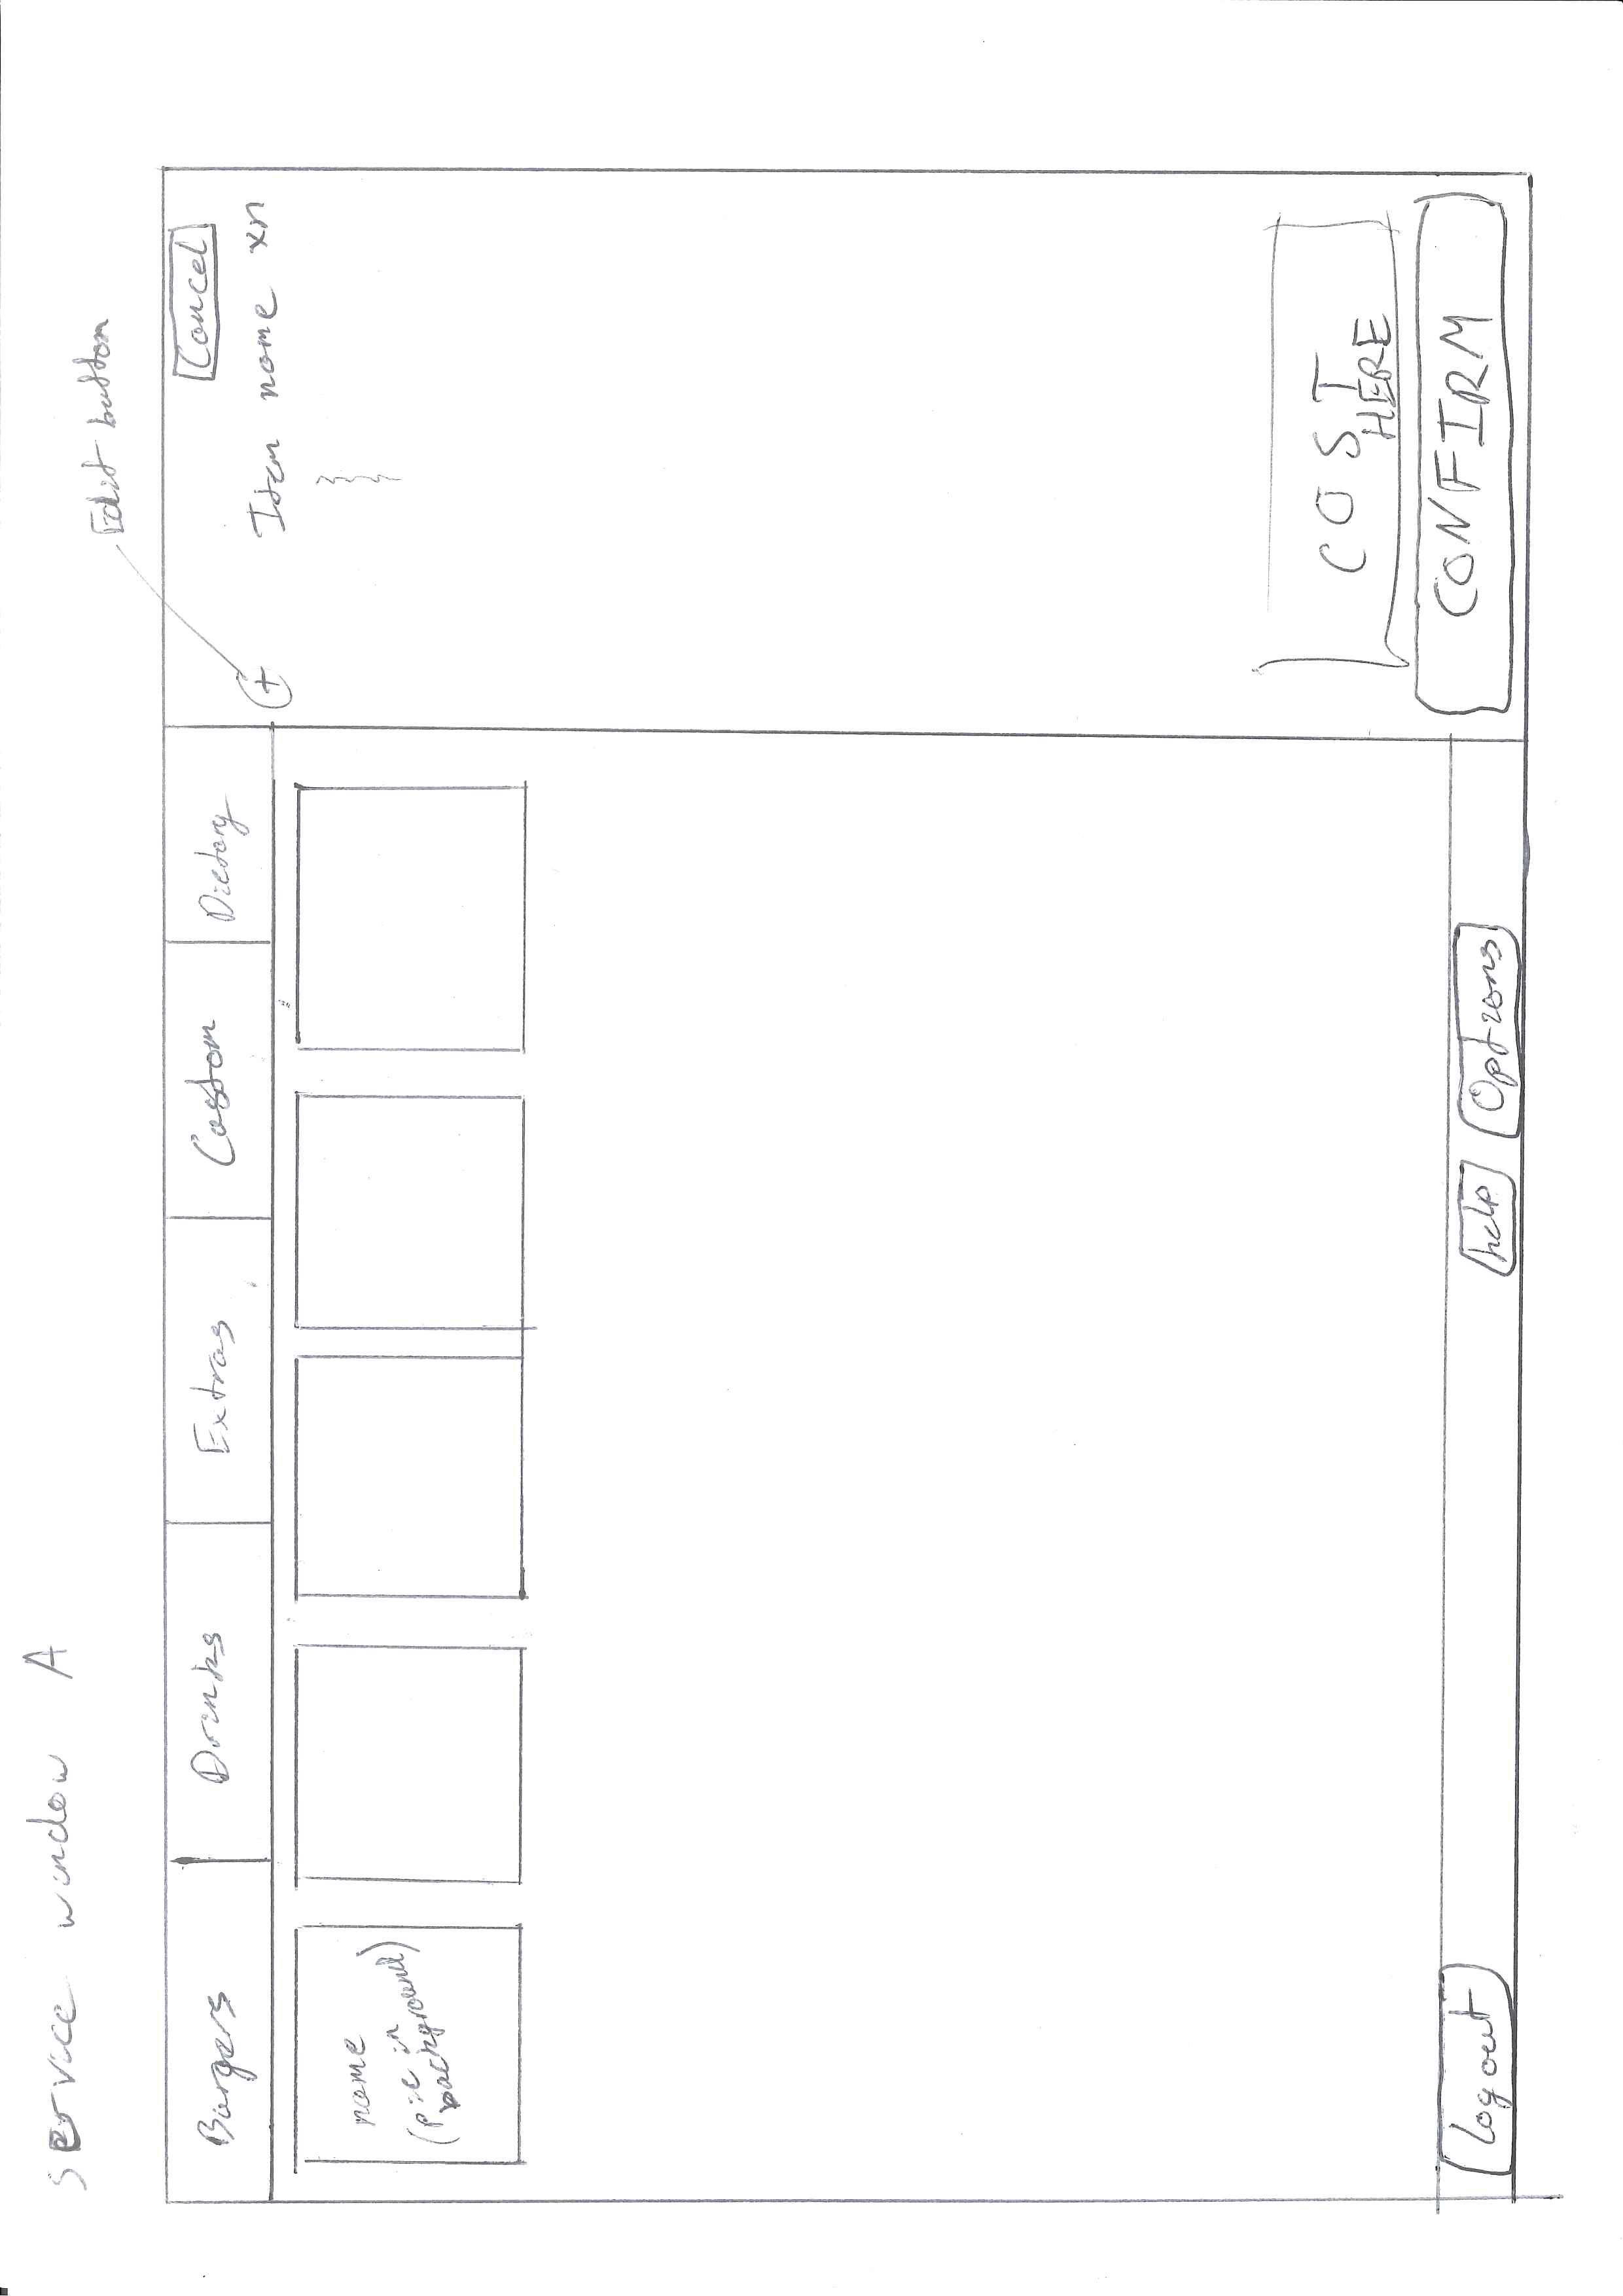
\includegraphics[width=100mm,angle=-90]{images/Wireframe_drafts/Service_window_A.jpg}
	\caption{Initial wireframe design of the order screen}
	\label{fig:Service_window_A}
\end{figure}

Figure \ref{fig:Service_window_A} shows a first draft of the order/service window. The main idea behind this design was to have large buttons for each item and a tabbed menu selector along the top for selecting categories. It also includes the idea of having an edit button for each item in the order. The other initial warframe concepts can be found in appendix A.

After doing some initial wireframes it was decided that going out and surveying some end users to find out what is important in a POS system would allow us to ensure that further development worked towards bettering the design. To such ends we talked to the Reboot cafe and the doughnut food truck on campus. The full questions and answers can be found in the apendix under user serveys as well as pictures of what each vendor currently has for their point of sales system.

After the serveys there were a few key points that were identified towaords moving forward. The first point was that as long as the system does not get in the way of their work it is a positive addition. The second key point was that it needs to be simple to use and that over complicating things would be a potential pit fall. It was also worth noting that although the Reboot cafe had semi automatic stock managment that gave them a end of day tally for use in restocking, the doughnut truck did not and all of their stock management was by eye. Finally we noticed whilst talking to the staff at the Reboot cafe that their system allowed them to colour code buttons by having their cold drinks using blue buttons and their coffees using brown buttons.

After this feedback from some end users more in depth GUI prototypes were developed using the online tool moqups. During this time we also took inspiration from the Reboot cafe and decided to colour code each of the item buttons to help with usability.

\begin{figure}[ht]
	\centering
	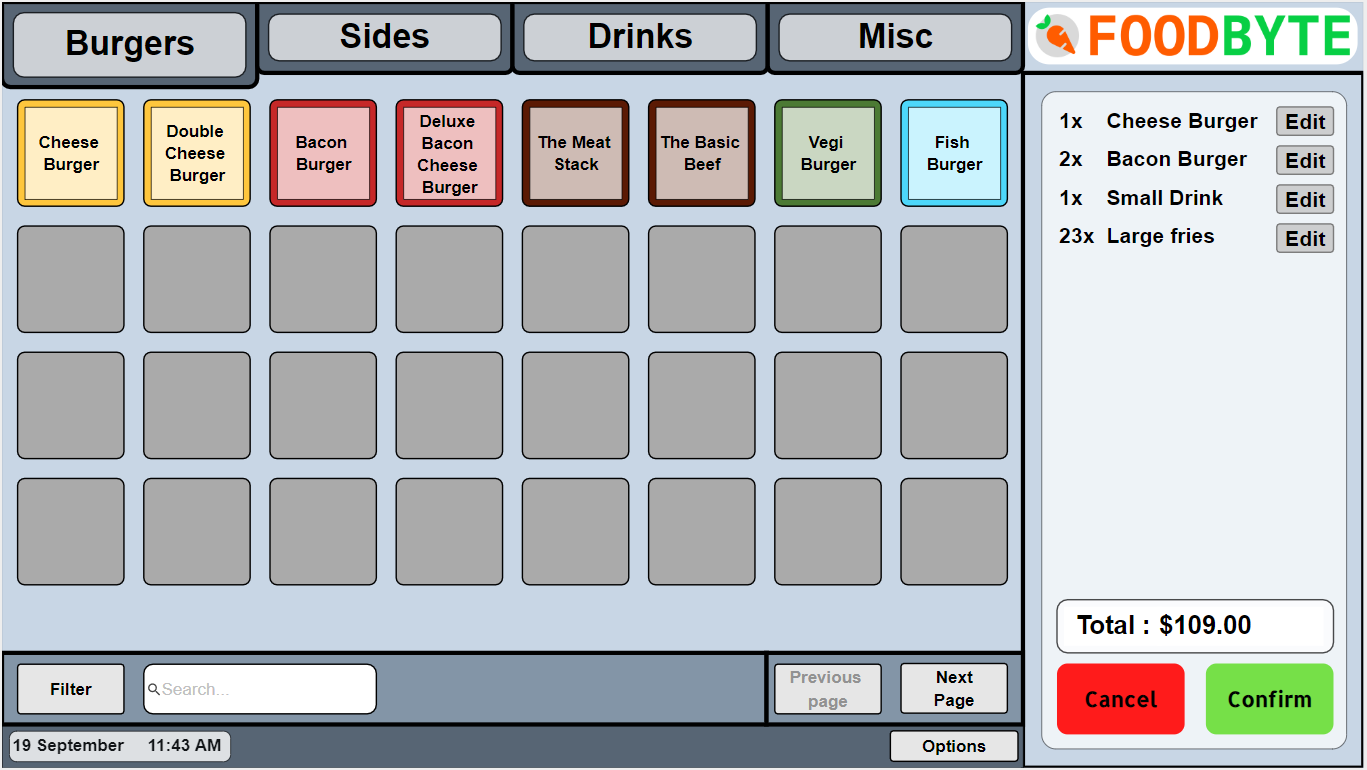
\includegraphics[width=150mm]{images/GUI_prototypes/Order_screen.PNG}
	\caption{Refined mock up of the order screen}
	\label{fig:order_screen_moqueup}
\end{figure}

In this GUI prototype (see figure \ref{fig:order_screen_moqueup}) several of the features, quality requirements and their use cases have been taken into consideration. Each item has a large button that is colour coded based on what it is (ie. cheese based/featuring items are yellow). This helps with the useability of the GUI (QR3) as well as directly implementing the ability to add an item to the current order (FR4). There is a clear and large cancel button to allow for the canceling of orders (FR6). The running total cost of the order is clearly displayed above the order confirmation button (FR3). The order confirmation button opens a popup for the order confirmation where, if payment is via cash, the change can be calculated (FR2). Each item in the current order has an edit button to allow for items to be edited (FR8, FR9). It can also be noted that there are selectable tabs for different categories as well as options to search and/or filter items. The date and time is displayed in the bottom left as this is a convenient feature to have during service. The next/previous page buttons are to allow for an overflow of items as page switching can be more reliable than scrolling (QR2). Finally there is an “Options” button that opens a popup with access to the management side of the application as well as the ability to modify aspects of the service side (ie. prices). The options popup also has a button to bring up an order history to facilitate providing refunds (FR7).
The prototype sub windows and popups related to the order screen can be found in the appendices.

\begin{figure}[ht]
	\centering
	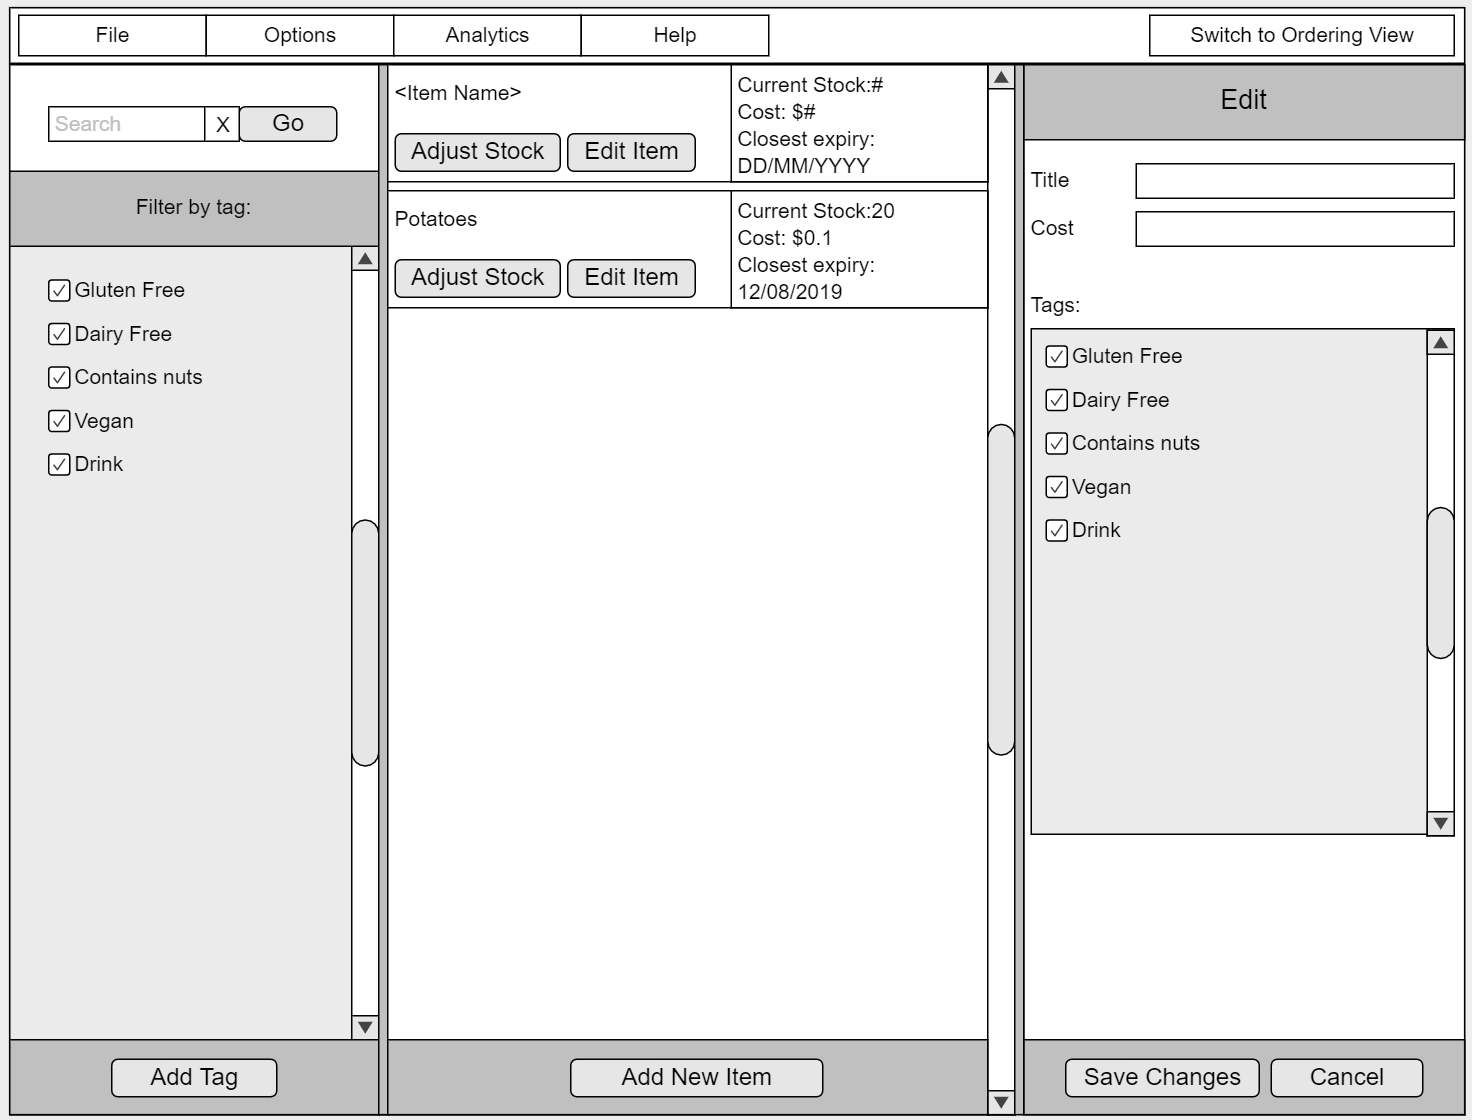
\includegraphics[width=150mm]{images/GUI_prototypes/Inventory_screen.png}
	\caption{Refined mock up of the inventory management screen}
	\label{fig:management_screen_moqueup}
\end{figure}

Figure \ref{fig:management_screen_moqueup}) shows a prototype design for the Inventory management system that features tools for stock management and product management. On the left there are options for filtering and searching items which will appear in the middle (FR16, FR19). Items can be added with the “Add New Item” button in the middle (FR20, FR18, FR10). Each item will have the current quantity displayed as well as the cost of the item and nearest expiry date, this will be alongside buttons to adjust stock level and edit item (FR20, FR14, FR24). On the right is the edit screen for editing a selected item, this could also be used for creating new items (FR13, FR10). At the top there are buttons for file which would allow for import/export (FR25, FR26). There is also a button to switch back to operational view and a button to switch to an analytics view (FR21, FR23).